\documentclass[../../main/main.tex]{subfiles}
\graphicspath{{./figures/}}

\makeatletter
\renewcommand{\@chapapp}{Optique -- chapitre}
\makeatother

% \toggletrue{student}
% \HideSolutionstrue

\begin{document}
\setcounter{chapter}{2}
\setlength{\columnseprule}{0pt}

\chapter{\switch{Correction du TD}{TD~: Miroir plan et lentilles minces}}

\section{Constructions optiques de lentilles}

Construisez les images par la lentille des objets suivants. On donnera à chaque
fois la nature de l'objet et de l'image.

\subsection{Pour une lentille convergente}
\switch{
	\begin{enumerate}
		\item Objet avant le foyer objet~;
		\item Objet sur le foyer objet~;
		\item Objet entre le foyer objet et la lentille~;
		\item Objet après la lentille~;
		\item Faisceau parallèle à l'axe optique~;
		\item Rayon quelconque incliné par rapport à l'axe optique.
	\end{enumerate}
}{
	\begin{multicols}{2}
		\begin{enumerate}
			\item ~\smallbreak
			      \vspace*{-20pt}
			      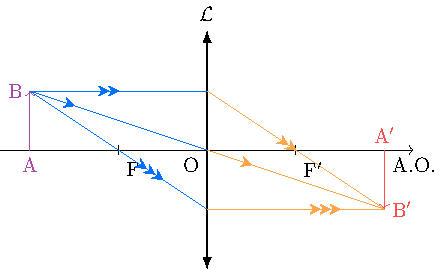
\includegraphics[width=\linewidth]{convAF}
			      Ces rayons, issus d'un \underline{objet réel}, se croisent après la
			      lentille~: on a un faisceau émergent \underline{convergent} qui
			      donne une \underline{image réelle}.
			\item ~\smallbreak
			      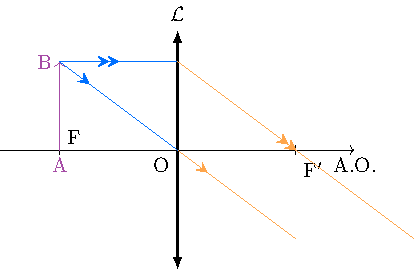
\includegraphics[width=\linewidth]{convBF}
			      À partir d'un \underline{objet réel}, on obtient des rayons
			      \underline{parallèles} qui donnent une \underline{image à l'infini}.
			      \columnbreak
			\item ~\smallbreak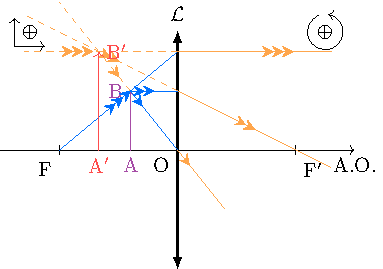
\includegraphics[width=\linewidth]{convCF}
			      Ici, l'objet est \underline{réel} mais donne un faisceau émergent
			      \underline{divergent}, donnant donc une image \underline{virtuelle}.
			\item ~\smallbreak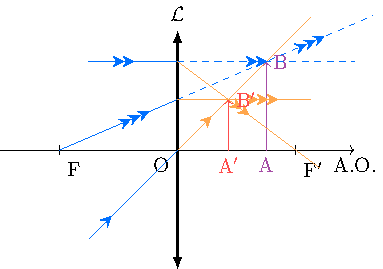
\includegraphics[width=\linewidth]{convDF}
			      On part d'un \underline{objet virtuel}. Les rayons partant de la
			      gauche du système passent par $B$, mais une fois arrivés à la
			      lentille on continue les traits en pointillés pour montrer que ce
			      sont des rayons virtuels. Le faisceau émergent est
			      \underline{convergent}, donnant lieu à une \underline{image réelle}.
			      \columnbreak
			\item ~\smallbreak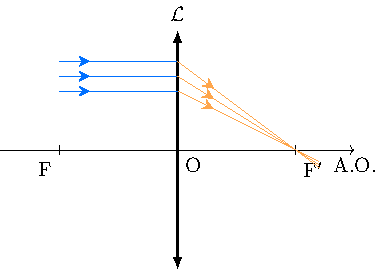
\includegraphics[width=\linewidth]{convHF}
			      Ici, l'objet est \underline{réel} et donne un faisceau émergent
			      \underline{convergent}, donnant donc une image \underline{réelle}.
			\item ~\smallbreak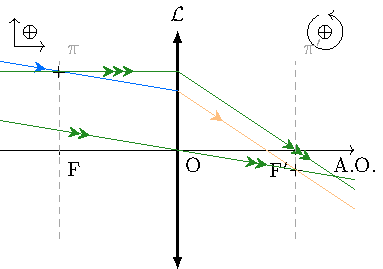
\includegraphics[width=\linewidth]{convQQE}
			      On n'a qu'un seul rayon, donc pas d'intersection~: aucune idée de la
			      nature de l'objet/image.
		\end{enumerate}
	\end{multicols}
}


\subsection{Pour une lentille divergente}
\switch{
	\begin{enumerate}
		\item Objet avant le foyer image~;
		\item Objet entre le foyer objet et la lentille~;
		\item Objet sur le foyer objet~;
		\item Objet après le foyer objet~;
		\item Faisceau parallèle à l'axe optique~;
		\item Rayon quelconque incliné par rapport à l'axe optique.
	\end{enumerate}
}{
	\begin{multicols}{2}
		\begin{enumerate}
			\item ~
			      \smallbreak
			      \vspace*{-20pt}
			      \begin{center}
				      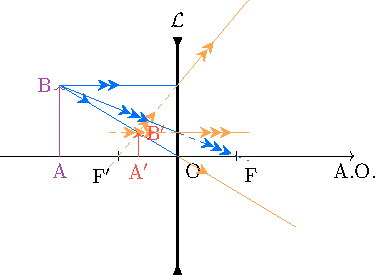
\includegraphics[width=\linewidth]{divAF}
			      \end{center}
			      Ces rayons, issus d'un \underline{objet réel}, se croisent avant la
			      lentille~: on a un faisceau émergent \underline{divergent} qui
			      donne une \underline{image virtuelle}.

			\item ~\smallbreak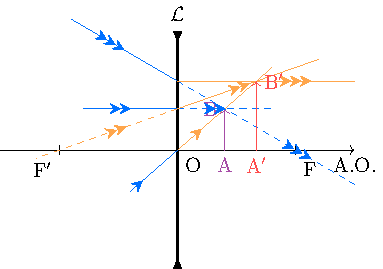
\includegraphics[width=\linewidth]{divBF}
			      À partir d'un \underline{objet virtuel}, on obtient des rayons
			      \underline{convergents} qui donnent une \underline{image réelle}.

			\item ~\smallbreak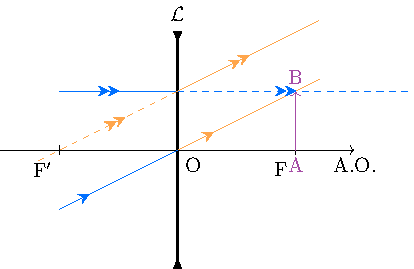
\includegraphics[width=\linewidth]{divCF}
			      Ici, l'objet est \underline{virtuel} et donne un faisceau émergent
			      \underline{parallèle}, donnant donc une image \underline{à l'infini}.
			\item ~\smallbreak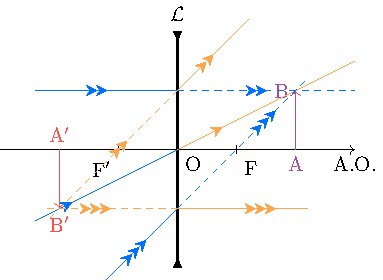
\includegraphics[width=\linewidth]{divDF}
			      On part d'un \underline{objet virtuel}. Le faisceau émergent est
			      \underline{divergent}, donnant lieu à une \underline{image virtuelle}.
			      \columnbreak
			\item ~\smallbreak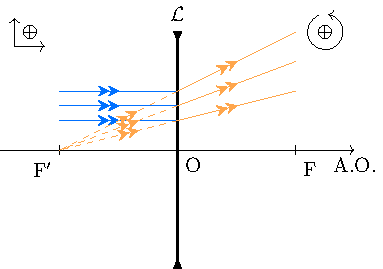
\includegraphics[width=\linewidth]{divHF}
			      Ici, l'objet est \underline{réel} et donne un faisceau émergent
			      \underline{divergent}, donnant donc une image \underline{virtuelle}.
			\item ~\smallbreak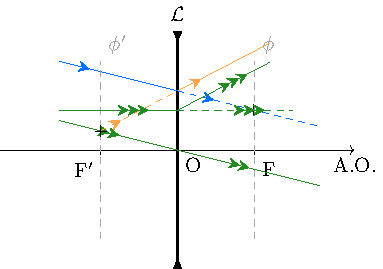
\includegraphics[width=\linewidth]{divQQE}
			      On n'a qu'un seul rayon, donc pas d'intersection~: aucune idée de la
			      nature de l'objet/image.
		\end{enumerate}
	\end{multicols}
}

\section{Constructions optiques de miroirs}
\switch{
	Dans chacune des situations suivantes, déterminer la nature des faisceaux,
	nommer les intersections dessinées, compléter la marche des rayons lumineux et
	commenter la nature de l'objet et de l'image.
	\begin{center}
		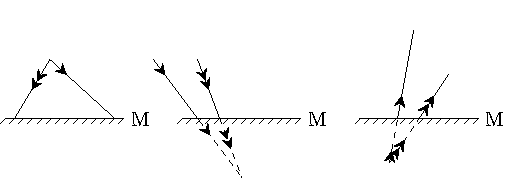
\includegraphics[height=4cm]{miroir_plan}
	\end{center}
}{
	\begin{tcb}[tabularx={Y|Y|Y}](data){Schéma}
		&&\\
		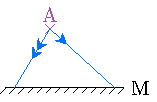
\includegraphics{td3-2-1a} &
		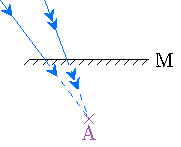
\includegraphics{td3-2-2a} &
		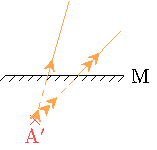
\includegraphics{td3-2-3a}\\
		Les rayons, incidents, se coupent avant le miroir. &
		Les rayons, incidents, se coupent après le miroir. &
		Les rayons, émergents, se coupent après le miroir.\\
	\end{tcb}
	\begin{tcbraster}[raster columns=2, raster equal height=rows]
		\begin{tcb}[](ques){Résultat attendu}
			Construire les objets et images avec les règles du miroir plan.
		\end{tcb}
		\begin{tcb}[](tool)'r'{Outils}
			Image par miroir plan = symétrique. Objet à intersection des indicents,
			image intersection émergents.
		\end{tcb}
	\end{tcbraster}
	\begin{tcb}[tabularx={Y|Y|Y}](appl){Application}
		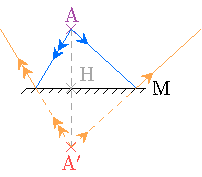
\includegraphics{td3-2-1b} &
		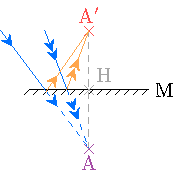
\includegraphics{td3-2-2b} &
		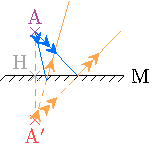
\includegraphics{td3-2-3b}\\
		Le symétrique de A donne A' où les rayons émergents se croisent. &
		Le symétrique de A donne A' où les rayons émergents se croisent. &
		Le symétrique de A' donne A où les rayons incidents se croisent.\\
		A est réel, A' virtuel. &
		A est virtuel, A' réel. &
		A est réel, A' virtuel.\\
	\end{tcb}
}

\section{Vidéoprojecteur}

\switch{
	On modélise l'objectif d'un vidéoprojecteur par une lentille mince convergente
	de distance focale de \SI{5.0}{cm}. L'objet transverse a une hauteur de
	\SI{24}{mm} et l'écran se situe à \SI{4.0}{m} de la lentille. Déterminer la
	position, la nature de l'objet ainsi que la taille de l'image.
}{
	\begin{tcb}[sidebyside, sidebyside align=center](data){Données}
		\begin{enumerate}
			\item $(\ABr) = \SI{24}{mm}$~: «~l'objet est transverse a une hauteur de
			      $\SI{24}{mm}$~»~;
			\item $\OAp = \SI{+4.0}{m}$~: «~l'écran se situe à $\SI{4.0}{m}$~»
			      (c'est là que se forme l'image, c'est donc la position de A')~;
			\item $\OFp = \SI{+5.0}{cm}$.
		\end{enumerate}
		\tcblower
		\begin{center}
			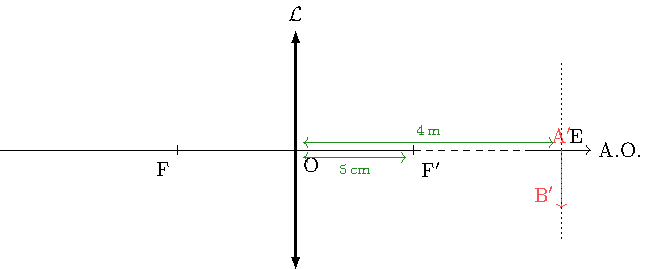
\includegraphics[width=\linewidth]{videoproj_plain}
		\end{center}
	\end{tcb}
	\begin{tcbraster}[raster columns=2, raster equal height=rows]
		\begin{tcb}(ques){Résultats attendus}
			\begin{enumerate}
				\item Que vaut $ \OA$~?~: «~Déterminer la position et la nature de
				      l'objet~» (O est bon point d'intérêt à partir duquel on peut
				      mesurer des distances, et selon la valeur \underline{algébrique} de
				      $\OA$ on saura de quel côté de la lentille l'objet se situe,
				      et donc son caractère virtuel ou réel)~;
				\item Que vaut $\ABp$~?~: «~Déterminer [...] la taille de l'image~».
			\end{enumerate}
		\end{tcb}
		\begin{tcb}(tool)'r'{Outils du cours}
			\begin{enumerate}
				\item Relation de conjugaison pour une lentille mince~:
				      \[ \boxed{ \frac{1}{\OFp} = \frac{1}{\OAp} - \frac{1}{\OA}}\]
				\item Grandissement pour une lentille mince~:
				      \[\boxed{\g = \frac{\ABp}{\AB} = \frac{\OAp}{\OA}}\]
			\end{enumerate}
		\end{tcb}
	\end{tcbraster}
	\begin{tcb}[breakable, sidebyside](appl){Application}
		\begin{enumerate}
			\item De la relation de conjugaison, on a~:
			      \[\OA = \left[ \frac{1}{\OAp} - \frac{1}{\OFp} \right]^{-1}\]
			      Et avec les données,
			      \[ \boxed{\OA = \SI{- 5.0}{cm}}\]
			      Ainsi, on a un \underline{objet réel} situé à 5 centimètres à gauche de
			      la lentille.
		\end{enumerate}
		\tcblower
		\begin{center}
			\begin{enumerate}[start=2]
				\item De l'expression du grandissement, on a~:
				      \[\ABp = \AB\times\frac{\OAp}{\OA}\]
				      Et avec les données,
				      \[ \boxed{\ABp = \SI{- 1.9}{m}} \]
			\end{enumerate}
			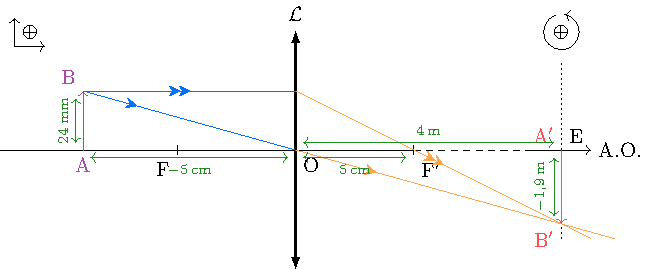
\includegraphics[width=\linewidth]{videoproj}
		\end{center}
	\end{tcb}

	\begin{tcb}(rema){Remarque}
		Attention, comme on a qu'un seul chiffre significatif, on a $\OA =
			\SI{-5}{cm}$, ce qui semble correspondre à la position de $F$, mais en
		réalité ce n'est qu'une approximation numérique. Comme $\OAp \gg \OFp$, le
		résultat numérique est proche de $-\OFp$, mais il est évident que si l'objet
		était en effet au foyer objet, le vidéoprojecteur ne formerait pas l'image
		sur l'écran mais à l'infini.
	\end{tcb}
}

\section{Œil réduit et accommodation}
\switch{
	Le cristallin de l'œil est assimilable à une lentille mince de distance focale
	variable (accommodation). L'image, pour être nette, doit se former sur la rétine
	qui est située à \SI{22.3}{mm} du cristallin. Lorsque l'œil n'accommode pas
	(cristallin au repos), il voit nettement un objet situé à l'infini. Lorsqu'il
	accommode au maximum, il voit nettement un objet jusqu'à \SI{25}{cm} (valeur
	moyenne).
	\begin{enumerate}
		\item Quelles sont la vergence et la distance focale du cristallin lorsque
		      l'œil voit nettement un objet placé à \SI{25}{cm}~? À l'infini~?
		\item On observe nettement un objet de \SI{10}{cm} de haut placé à
		      \SI{1}{m}. Quelle est la vergence du cristallin~?
		\item Dans ces conditions d'observation, quels sont le sens et la taille de
		      l'image formée sur la rétine~?
	\end{enumerate}
}{
	\begin{tcb}(data){Données}
		\begin{minipage}{0.5\linewidth}
			\begin{enumerate}
				\item Rétine = écran,
				      cristallin = lentille~;
				\item Au repos, A à l'infini~;
				\item Au \textit{proximum}, A à \SI{25}{cm}
				      ($\OA = \SI{-25}{cm}$).
			\end{enumerate}
		\end{minipage}
		\begin{minipage}{0.5\linewidth}
			\begin{center}
				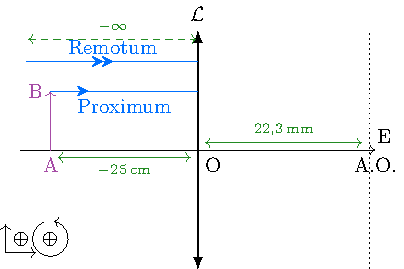
\includegraphics[width=\linewidth]{oeil_plain}
			\end{center}
		\end{minipage}
	\end{tcb}

	\begin{tcbraster}[raster columns=3, raster equal height=rows]
		\begin{tcb}(ques){Résultats attendus}
			\begin{enumerate}
				\item $\OFp _\mathrm{repos}$~?
				\item $\OFp _\mathrm{accomodation}$~?
			\end{enumerate}
		\end{tcb}
		\begin{tcb}[raster multicolumn=2](tool)'r'{Outils du cours}
			Relation de conjugaison pour une lentille mince, avec $\OAp = \obar{\rm
					OE} = \SI{22.3}{mm}$ (le principe d'un écran c'est que l'image se forme
			dessus~!!) et $\frac{1}{\OA} = 0$ quand $\OA = -\infty$
		\end{tcb}
	\end{tcbraster}

	\begin{tcb}[breakable, sidebyside](appl){Résultats}
		\[ \boxed{\OFp_\mathrm{repos} = \SI{22.3}{mm}}\]
		\begin{center}
			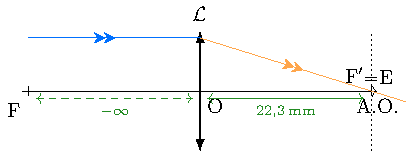
\includegraphics[width=\linewidth]{oeil_repos}
		\end{center}
		\tcblower
		\[ \boxed{\OFp_\mathrm{accomodation} = \SI{20.6}{mm}} \]
		\begin{center}
			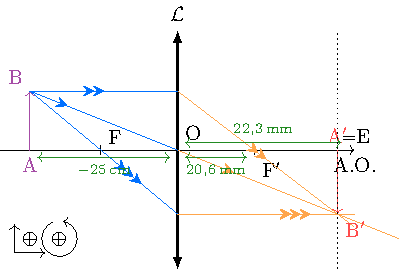
\includegraphics[width=\linewidth]{oeil_acco}
		\end{center}
	\end{tcb}
}

\section{Coin de miroir}
\switch{
	Un rayon lumineux pénètre dans un système optique composé de deux miroirs plans
	faisant un angle $\alpha$ entre eux. Il rentre parallèlement à un
	miroir et ressort du système en revenant sur lui-même par le même chemin
	optique après trois réflexions. Quelle est la valeur de $\alpha$~?
}{
	\noindent
	\begin{minipage}{0.48\linewidth}
		On compte 3 réflexions, et il doit revenir sur lui-même~: le rayon incident
		et le rayon émergent doivent faire le même angle avec la normale à BC.
		L'angle $i_2$ est également identique de $I$ à $J$ et de $J$ à $I$. Cela
		n'est vérifié que si la lumière est en incidence normale sur AB.

		Or, $i_1 = \frac{\pi}{2} - \alpha$, donc $i_2 = -i_1 =
			\alpha-\frac{\pi}{2}$. Pour avoir $i_2$ dirigé verticalement, il faut
		$-i_1+i_2 = -\frac{\pi}{2}$, autrement dit $2i_1 = \frac{\pi}{2}
			\Leftrightarrow i_1 = \frac{\pi}{4}$. Finalement, on trouve

		\begin{empheq}[box=\fbox]{equation*}
			\alpha = \SI[parse-numbers=false]{\frac{\pi}{4}}{rad}
		\end{empheq}
	\end{minipage}
	\hfill
	\begin{minipage}{0.48\linewidth}
		\begin{center}
			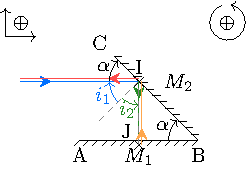
\includegraphics[width=\linewidth]{coin_mir}
			\captionof{figure}{Schéma du système}
			\label{fig:coin_mir}
		\end{center}
	\end{minipage}
}

\section{Étude d'un rétroprojecteur}
\switch{
	\noindent
	\begin{minipage}[c]{.58\linewidth}
		Un rétroprojecteur est un ensemble lentille-miroir, avec un miroir plan incliné
		à \ang{45;;} par rapport à la lentille. L'ensemble lentille-miroir est réglable
		en hauteur ($h$). On étudie un rétroprojecteur dont la lentille a une vergence
		de $\SI{2.0}{\delta}$, avec une distance lentille-miroir $d = \SI{10}{cm}$.
		\smallbreak
		On désire projeter un objet transparent AB sur un écran placé à $D =
			\SI{3.0}{m}$ de l'axe optique de la lentille.
		\begin{enumerate}
			\item Déterminer la distance $h$ permettant d'obtenir une image nette sur
			      l'écran.
			\item Calculer le grandissement.
		\end{enumerate}
	\end{minipage}
	\hfill
	\begin{minipage}[c]{.4\linewidth}
		~
		\begin{center}
			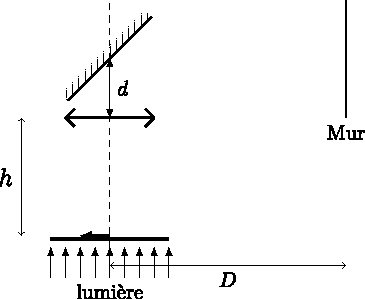
\includegraphics[width=\linewidth]{retroproj}
			\label{fig:retroproj}
		\end{center}
	\end{minipage}
}{
	\begin{enumerate}
		\item On a $\AB \opto{\Lc}{\Or} \ABb \opto{M}{\rm H} \ABp$, avec H le point
		      d'intersection entre le miroir plan et l'axe optique de la lentille.
		      L'image finale A' donnée par le miroir plan est telle que
		      \[
			      \boxed{\obar{\rm HA'} = \obar{\rm HA_1} = D}
		      \]
		      On a donc pour la lentille
		      \begin{empheq}[box=\fbox]{align*}
			      \obar{\rm OA_1} &= \obar{\rm OH} + \obar{\rm HA_1}
			      \\\Lra
			      \obar{\rm OA_1} &= d+D
		      \end{empheq}
		      On utilise la relation de conjugaison des lentilles minces en nommant
		      $V$ la vergence de la lentille~:
		      \begin{equation*}
			      V = \frac{1}{d+D} - \frac{1}{-h}
			      \Lra
			      \boxed{h = \frac{d+D}{V(d+D)-d}}
			      \qav
			      \left\{
			      \begin{array}{rcl}
				      d & = & \SI{10e-2}{m}    \\
				      D & = & \SI{3.0}{m}      \\
				      V & = & \SI{2.0}{m^{-1}}
			      \end{array}
			      \right.
		      \end{equation*}
		      Et l'application numérique donne
		      \begin{equation*}
			      \xul{h = \SI{60}{cm}}
		      \end{equation*}
		\item Le miroir plan a un grandissement de 1, donc le grandissement du
		      système est celui de la lentille~: on a $\gamma = \DS
			      \frac{\ABb}{\AB} = \frac{\obar{\rm OA_1}}{\OA}$, soit
		      \begin{empheq}[box=\fbox]{align*}
			      \gamma &= \frac{d+D}{-h}\\
			      \gamma &= -5.2
		      \end{empheq}
	\end{enumerate}
}

\end{document}
